\chapter{Experiment}
\section{Landing system}
The path system has successfully been tested in the field, where the result from two subsequent days will be presented. The landing plan that was test was only with a virtual net that was placed $26$ meters above the ground. The landing system has been tested in FBWA mode in ardupilot with guidance and control system developed by a fellow master student at the UAVlab. The navigation system used \gls{rtk-gps} with the compensator system enabled, which ensures that the positioning of the X can be assumed highly accurate. The result of the navigation system is presented in section \ref{ss:EXNavigation}.

The wind condition the first day had an windspeed at $8-9 m/s$ from west, and the second day was calm wind conditions at $1 m/s$ from west. Hence the performance of system was tested with two different wind condition, where one strained the system and the other could be considered ideal conditions. The criteria used to indicate if the X8 would have hit the net is given in table \ref{tb:NetCriteria}, which is related to a net with the dimensions 3 meter height and 5 meter width.
\begin{table}[H]
\centering
\begin{tabular}{| l | l |}
\hline
\textbf{Height acceptance}	& \textbf{Cross track error acceptance}	\\ \hline
$\pm1.5$					& $\pm2.5$								\\ \hline
\end{tabular}
\caption{Net hit acceptance criteria}
\label{tb:NetCriteria}
\end{table} 
\newpage
\subsection{Day 1}
The wind condition for the first day was $8-9 m/s$ from west, which is parallel to the runway such that a head wind landing is possible. The \gls{uav} was set to loiter at a fixed point, from which the landing plan was generated. The lateral path of the \gls{uav} is shown in figure \ref{Fig:NorthEast31mai103029} and longitudinal path in \ref{Fig:Height31mai103029} with desired path and height respectfully.

The behaviour of the lateral path shown in figure \ref{Fig:NorthEast31mai103029} indicates that the lateral guidance system is struggling to hold the line when flying in the crosswind. When exiting the overshoot may cause the \gls{uav} to leave the line of sight of the pilot, in which case the only method of monitoring the \gls{uav} is over a radio link which can experience drop out. The behaviour of the \gls{uav} when flying keeps ocislating around the straight line path, which is undesired during the finale stage of the landing plan. This behaviour can be reduced by lowering the lookahead distance in the lateral guidance system, which increased the performance during the final stage as shown in figure \ref{Fig:NorthEast31mai105034}.  

The longitudinal guidance system used outputs a desired heigh which lags behind the desired path due to a smoothing filter which is used to remove the discontinue between two line segments. The filter currently used will only converge to a constant height value, such that the net impact angle has to zero in order for the longitudinal guidance system to converge to the desired path height. A new landing plan, shown in figure \ref{Fig:Height31mai31mai105034} and \ref{Fig:NorthEast31mai105034}, was generated with the net impact angle $\gamma_n = 0$ which gave a better performance from the height guidance system. However this results in that the glide slope is the only part of the landing path where the height can be reduced, which will cause a problem when attempting to land in a real net. This is due to the length restriction of both the airfield and the operational area where the \gls{uav} is visible for the pilot. With the current landing plan and a landing direction from east the minimum height at which the \gls{uav} can starts its landing path is set to $56 m$ above ground. 
\newpage
\begin{figure}[H]
\begin{subfigure}[H]{1\textwidth}
	\centering
		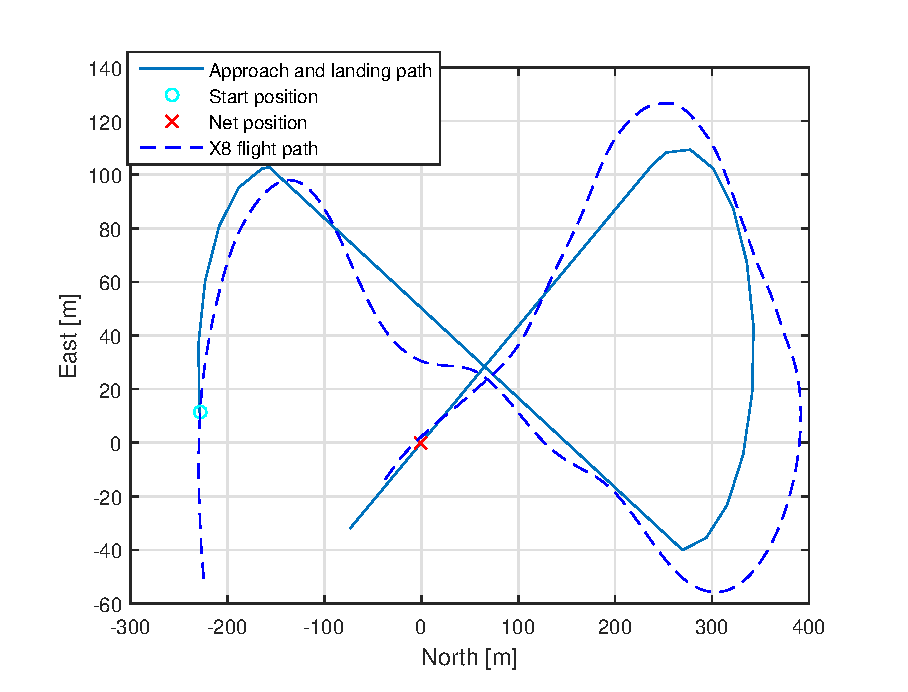
\includegraphics[width=1\textwidth]{figs/Experiment/NorthEast31mai103029.eps}
		\caption{North-East plot of a landing plan}
		\label{Fig:NorthEast31mai103029}
\end{subfigure}
\begin{subfigure}[H]{1\textwidth}
		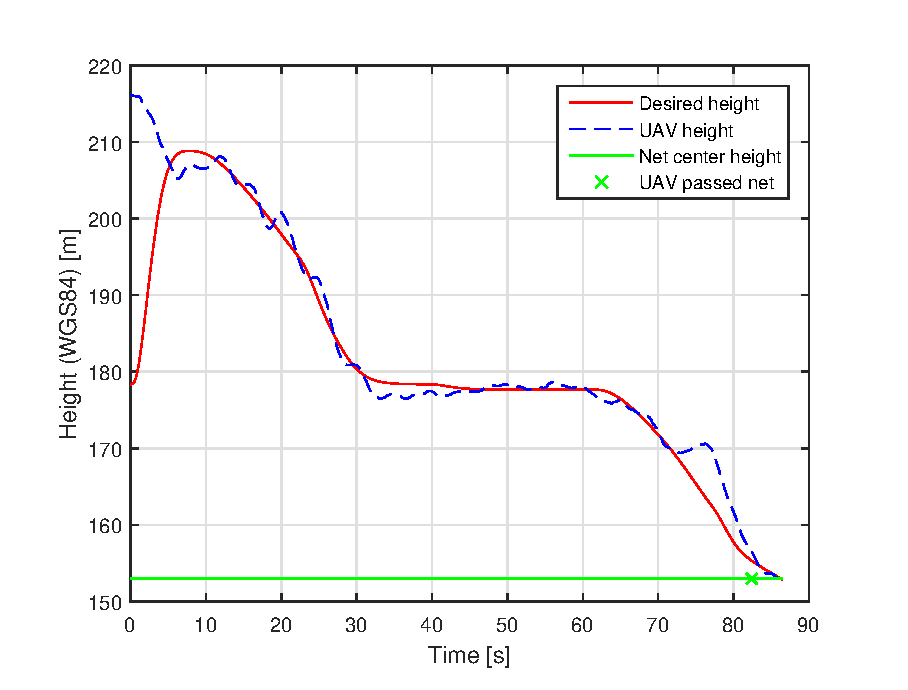
\includegraphics[width=1\textwidth]{figs/Experiment/Height31mai103029.eps}
		\caption{Height profile of landing plan with $3 \deg$ net impact angle}
		\label{Fig:Height31mai103029}
\end{subfigure}
\end{figure}
The performance form the lateral controller was increased by lowering the lookahead distance parameter. However the \gls{uav} still have ocilatoric behaviour along the straight line parts, with a large overshoot in the final turn.


\newpage
\begin{figure}[H]
\begin{subfigure}[H]{1\textwidth}
	\centering
		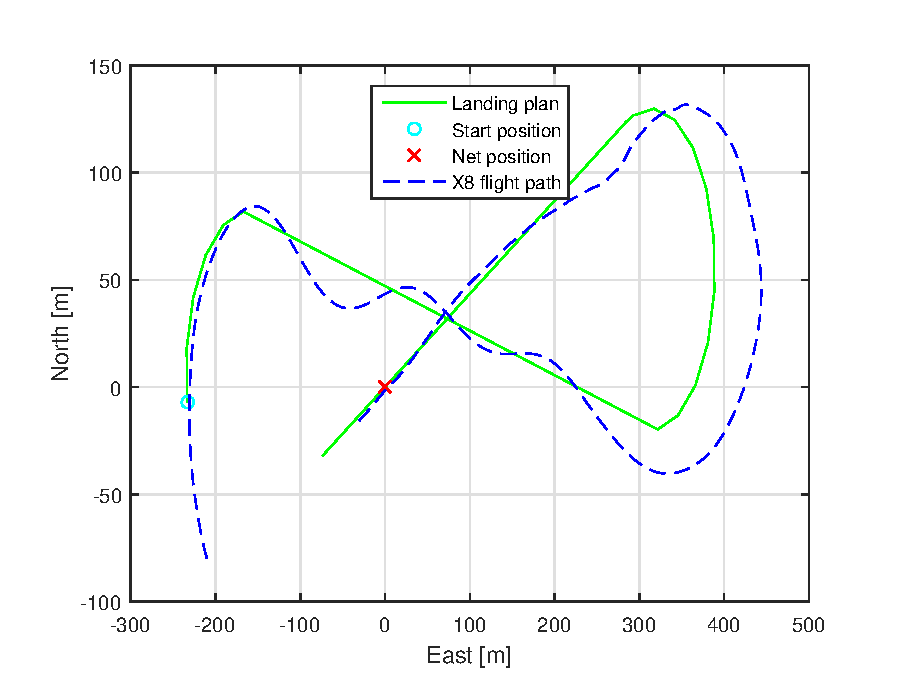
\includegraphics[width=1\textwidth]{figs/Experiment/NorthEast31mai105034.eps}
		\caption{North-East plot of a landing plan}
		\label{Fig:NorthEast31mai105034}
\end{subfigure}
\begin{subfigure}[H]{1\textwidth}
		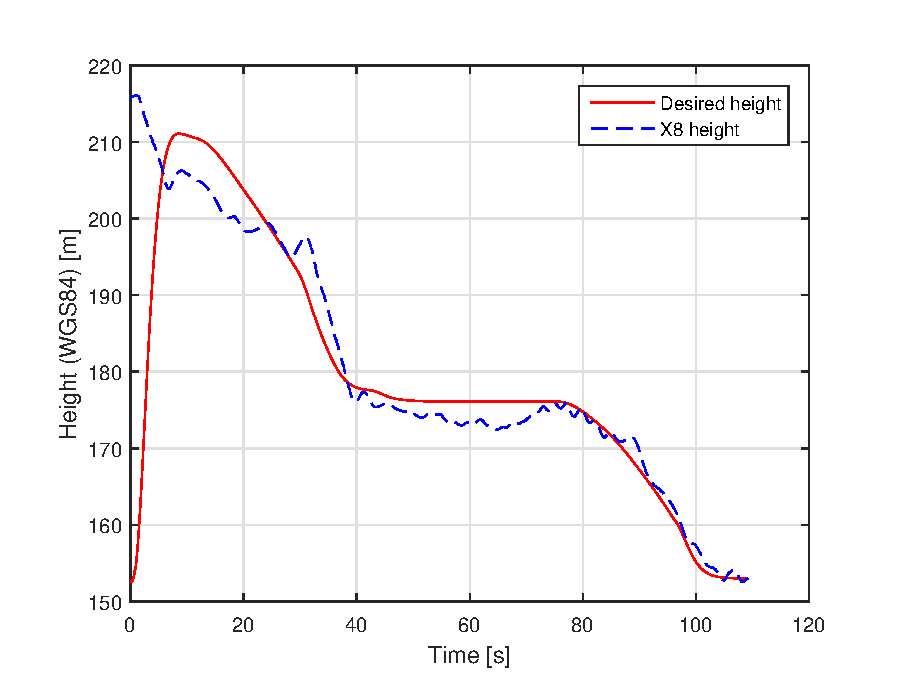
\includegraphics[width=1\textwidth]{figs/Experiment/Height31mai105034.eps}
		\caption{Height profile of landing plan with $0 \deg$ net impact angle}
		\label{Fig:Height31mai31mai105034}
\end{subfigure}
\end{figure}
\subsubsection{Summary of day 1}
The result from the first day was affected with strong wind condition, in which the \gls{uav} struggeled to stay on the path. The mean height and cross track error is listed in table \ref{tb:Day1HeightCrossTrack}, where the first column indicate the number of the landing attempt.
\begin{table}[H]
\centering
\begin{tabular}{| l | l | l |}
\hline
\textbf{Nr.} 	& \textbf{Mean height error} 	& \textbf{Mean cross track error}  \\ \hline
$1$				& $1.5$							& $6.1$								\\ \hline
$2$				& $2.6$							& $6.7$								\\ \hline
$3$				& $0.9$							& $5.5$								\\ \hline
$4$				& $0.1$							& $2.8$								\\ \hline
$5$				& $1.7$							& $2.0$								\\ \hline
$6$				& $1.3$							& $6.8$								\\ \hline
$7$				& $1,8$							& $9.1$								\\ \hline
$8$				& $1.2$							& $8.2$								\\ \hline
$9$				& $1.9$							& $5.9$								\\ \hline
$10$			& $1.5$							& $4.4$								\\ \hline
$11$			& $1.5$							& $1.4$								\\ \hline
\end{tabular}
\caption{Mean height and cross track error from day 1}
\label{tb:Day1HeightCrossTrack}
\end{table}
\begin{table}
\centering
\begin{tabular}{| p{0.5cm} | p{1cm} | p{1cm} | p{3.5cm} | p{3cm} | p{1cm} |}
\hline
\textbf{Nr.}	& \textbf{Height error}	& \textbf{Cross track error}& \textbf{Height acceptance}& \textbf{Cross track error acceptance}	& \textbf{Net hit}\\ \hline
$1$				& $2.8 m $	& $2.1 m$	& X								& OK									& X	\\ \hline
$2$				& $2.7 m$	& $-4.5$	&X								& X										& X					\\ \hline
$3$				& $0.9 m$	& $-1.6 m$	&OK							& OK									& OK				\\ \hline
$4$				& $0 m$		& $5.4 m$	&OK							& X										& X					\\ \hline
$5$				& $0.8 m$	& $5.3 m$	&OK							& X										& X					\\ \hline
$6$				& $2.1 m$	& $-1.6 m $	&X								& OK									& X					\\ \hline
$7$				& $0.7 m$	& $2.3 m $	&OK							& OK									& OK				\\ \hline
$8$				& $-1.5 m $ & $-5.4 m $	&X								& X										& X					\\ \hline
$9$				& $1.9 m$	& $0.8 m $	&X								& OK									& X					\\ \hline
$10$			& $0.3 m$	& $1.1 m $	&OK							& OK									& OK				\\ \hline
$11$			& $-1.3 m$	& $0.15 m $	&OK							& OK									& OK				\\ \hline
\end{tabular}
\end{table}
\subsection{Day 2}
The wind condition on the second day was calm, which allowed for testing the performance of the landing system under ideal conditions.
\begin{table}[H]
\centering
\begin{tabular}{| l | l | l |}
\hline
\textbf{Nr.} 	& \textbf{Mean height error} 	& \textbf{Mean cross track error}  \\ \hline
$1$				& $2.2$							& $3.8$								\\ \hline
$2$				& $1.2$							& $3.4$								\\ \hline
$3$				& $0.9$							& $-1.8$							\\ \hline
$4$				& $2.5$							& $-0.2$							\\ \hline
$5$				& $3.0$							& $0.3$								\\ \hline
$6$				& $1.6$							& $0.2$								\\ \hline
$7$				& $1,9$							& $-2.3$							\\ \hline
$8$				& $1.9$							& $-0.1$							\\ \hline
\end{tabular}
\caption{Mean height and cross track error from day 2}
\end{table}
Observation from the airfield is that the minimum altitude of the \gls{uav} during a landing from east is $56 m$ with the current landing path design. The height controller used saturates in the desired pitch when trying to follow slope at $6 \deg$. A landing path with the maximum slope angle of $6 \deg$ would require a landing path of $700 m$. The the current length of the glide slope the slope angle has to be $11 \deg$. However with a large slope angle the \gls{uav} will quickly gain speed, which will cause a large overshoot at the desired height if not accounted for.

The lateral controller in DUNE performed satisfying during calm wind condition, where the overshoot in the start of each landing plan could have been cause by a bug in the value of the desired height value. However the performance during stronger wind condition cause that the controller to struggle, which is visible during the $180 \deg$ turn. The rapid transition of points during a turn affect the controller with having to recalculate the bank angle during the turn, where a better solution would be to try to keep the bank of the \gls{uav}. This would require the controller to know all the point in the follow path manoeuvre, without breaking the modular boundaries in the DUNE environment.
\section{Navigation}\label{ss:EXNavigation}
The navigation system was tested in both a X8 and in a multicopter system.

\subsection{Formation position}
The accuracy of the \gls{rtk-gps} position system was tested with two mutlicopter system, with the goal of measuring the distance between them. During stationary conditions it was determined that \gls{rtk-gps} was highly accurate, and is required when performing a formation flight. The same principle is used in determining the net position, where the net nest apply \gls{rtk-gps} to determine it's own position. However currently the position has to manually be written to Neptus, which must change when performing a ship landing.
\subsection{Short loss compensator}
Include result when short loss was not in use. Compare to result when it's in use.

The short loss compensator bring the position solution from the pixhawk close enough to the \gls{rtk-gps} solution such that the navigation system does not lose its position. However a highly aggressive control system that attempt to keep the error at centimeter level is expected to react to the discontinues introduced from the compensator. All though currently it has not been concluded that the compensator cause problems for the control system, since failure has happen during demanding wind condition. 